% LaTeX Template for Project Report,
% It is advisable to learn the basics of LaTeX before using this template.
% A good resource to start with is http://en.wikibooks.org/wiki/LaTeX/
% Empty space after chapter/section/subsection titles can be used to insert text.
%
% Just compile this file after making all required changes.

\documentclass[12pt,a4paper]{report}
\usepackage[bookmarks, colorlinks=false, pdfborder={0 0 0}, pdftitle={Smart Traffic System Management using IOT}, pdfauthor={Hariharan K, Dhyan}, pdfsubject={Project Report}, pdfkeywords={report}]{hyperref} %for creating links in the pdf version and other additional pdf attributes, no effect on the printed document


%adjust your page margins here
\usepackage[top=0.8in, bottom=0.75in, left=1.25in,right=1in]{geometry} % setting the page alignment with this package

%To change line spacing in a specific environment you will use the second way, which is to add \usepackage{setspace} to the preamble and then you can make use of the command \singlespacing, \doublespacing, or \onehalfspacing to specify the line spacing for all sections and paragraphs until you sued another command to change it.
\usepackage{setspace} 

%for page borders use this package
\usepackage{fancybox}

%use this package to change the default chapter number and name display
\usepackage{titlesec}

%for embedding images
\usepackage[pdftex]{graphicx} 

%for proper url entries
\usepackage{url} 

%for set color to text
\usepackage[dvipsnames]{xcolor}

%for using Rs. symbol
\usepackage{tfrupee}

% Renewed commands to set the titles of various pages correctly.
\renewcommand\contentsname{\centering TABLE OF CONTENTS}
   \renewcommand\listfigurename{\centering LIST OF FIGURES}
   \renewcommand\listtablename{\centering LIST OF TABLES}
   \renewcommand\bibname{\centering REFERENCES}
   \renewcommand\appendixname{APPENDIX}

%to display chapter number left and chapter title center
\titleformat{\chapter}[display]
  {\normalfont\Large\bfseries}{\filright\chaptertitlename\ \thechapter}
  {20pt}{\Huge\filcenter}
	
\begin{document}
\renewcommand\bibname{References} %Renames "Bibliography" to "References" on ref page


\begin{titlepage}

\begin{center}
%\begin{framed}
\thispagestyle{empty}
\thisfancypage{%
  \setlength{\fboxsep}{10pt}\doublebox}{}

\vspace*{1\baselineskip}

\textcolor{Blue}{\LARGE{\textbf{Malnad College of Engineering}} }\\ 
\textcolor{Red}{\small{(An Autonomous Institution under Visvesvaraya Tecnological University, Belgaum)}}\\
\textcolor{Blue}{\large{\textbf{Hassan - 573202, Karnataka, India}}}\\[0.2in]


\includegraphics[width=0.18\textwidth]{./vtu_new.png}\\[0.2in]

\Large{\small{A PROJECT REPORT \\ ON}}\\
% Title
\textcolor{Red}{\Large{\textsc {\textbf{``SMART TRAFFIC CONTROL SYSTEM USING IOT"}}}}\\[0.1cm]
%Example
%\Huge{\textsc {\textbf{A case study on linux}}}\\[1.0cm]
\small \emph{Submitted in partial fulfillment of\\
        the requirements for the award of the degree of}
        \vspace{.2in}

       \textcolor{Blue}{{\bf Bachelor of Engineering \\in\\ Computer Science and Engineering}}\\[0.25cm]

\vspace{.2in}					
% Submitted by
\textcolor{Blue}{\normalsize Submitted by }\\

\begin{table}[h]
\centering
\begin{tabular}{lr}
\color{Blue}Hariharan K & \color{Red}4MC19CS050 \\
\color{Blue}Dhyan S Agni & \color{Red}4MC19CS043 \\ 
\end{tabular}
\end{table}


\vspace{.2in}
\textcolor{Blue}{Under the guidance of}\\
\textcolor{Red}{{\textbf{Mr. Shashidhara H V}}\\
Associate Professor}\\
\vspace{0.5cm}

\includegraphics[width=0.18\textwidth]{./mce_logo.png}\\[0.1in]

% Bottom of the page
% 
\includegraphics[width=0.18\textwidth]{./mce_logo.png}\\[0.1in]
\textcolor{Blue}{\Large{Department of Computer Science and Engineering}\\
\Large{Malnad College of Engineering}\\
\normalsize
Hassan - 573202, Karnataka, India\\}

\vspace{0.5cm}

\begin{table}[h]
\centering
\begin{tabular}{lllll}
\textcolor{Red}{Tel:} \textcolor{Blue}{08172-245093} & & \textcolor{Red}{Tel:} \textcolor{Blue}{08172-245317(Dept.)} & & \textcolor{Red}{URL:} \textcolor{Blue}{\href{https://www.mcehassan.ac.in/}{www.mcehassan.ac.in}}\\
\end{tabular}
\end{table}
\vspace{0.2cm}
\textcolor{Blue}{2022-2023}

%\end{framed}
\end{center}

\end{titlepage}
\newpage

\thispagestyle{empty}

\thisfancypage{%
  \setlength{\fboxsep}{10pt}\doublebox}{}

\begin{center}
    
\includegraphics[width=6in]{./images/signedCertificate.jpg}\\
\end{center}
\newpage
\vspace*{0.5\baselineskip}
\begin{center}
\thispagestyle{empty}
\LARGE{\textbf{ACKNOWLEDGEMENTS}}\\[0.5cm]
\end{center}
% \vspace{0.05cm}
\doublespacing

We present with immense pleasure this work titled \textbf{``Smart Traffic Control System Using IoT"}. An endeavour over a long period can be successful with the advice and support of many well wishers.

We take this opportunity to express our gratitude and appreciation
to all of them. The satisfaction and euphoria that accompany the successful completion of any
task would be incomplete without mentioning the people who made it possible. So,
with gratitude we acknowledge all those whose guidance and encouragement made to
successfully complete this project.

We would like to express sincere thanks to our Principal \textbf{Dr. Pradeep S}, Malnad
College of Engineering for his encouragement made to successfully completion of the
project work. We wish to express our gratitude to \textbf{Dr.Geetha Kiran A}, Professor and Head, Department of Computer Science \& Engineering for providing a good working environment and for her constant support and encouragement.

It gives great pleasure in placing on record a deep sense of gratitude to our guide
\textbf{Mr. Shashidhara H V}, Associate Professor, Department of Computer Science \& Engineering for his daily evaluation of the work and for providing us constant encouragement with his unflinching support and valuable guidance throughout this project.

We would also like to thank all the staff of Computer Science and Engineering department who have directly or indirectly helped us in the completion of the project work. At last we would hereby acknowledge and thank our parents who have been a source of inspiration and also instrumental in the successful completion of the project work. \\

\large{\hspace*{3.5in} Hariharan K(4MC19CS050)}\\
\large{\hspace*{3.7in} Dhyan S Agni(4MC19CS043)}\\



% Salutations to our beloved and highly esteemed institute ``Malnad College Of Engineering" for having well qualified staff and labs furnished with necessary equipment.

% The successful completion of any task would be incomplete without mentioning the people who have constantly guided and inspired for the project and the report generation.

% We avail this opportunity to thank all those people who have helped us in the whole process of completion of this project and the report.

% We would like to express our deepest gratitude to our mentor {\textbf{Prof. Shashidhara H V}},Department of Computer Science and Engineering for his daily evaluation of the work and for providing us constant encouragement with his unflinching support and valuable guidance throughout this project. We are indebted to him as he has considered us worthy of this project and invested his faith in us. It was a great privilege to work under him. We will take away a lot more than just the technical knowledge from him.We would also like to place our special thanks to Dr.C V Venkatesh, Principal,Dr Geetha Kiran A,HOD Computer science and Engineering department and all Panel members Mr. Shashidhara H V(Panel Head),Associate Professor, Mr.Vasanth Kumar N.T,Assistant Professor, Mrs.Harshitha S, Assistant Professor and Mrs.Nivyashree R, Assistant Professor Malnad College of Engineering for providing the opportunity and the facilities for the completion of our project.\\



% Salutations to our beloved and highly esteemed institute ``Malnad College Of Engineering" for having well qualified staff and labs furnished with necessary equipment.

% The successful completion of any task would be incomplete without mentioning the people who have constantly guided and inspired for the project and the report generation.

% We avail this opportunity to thank all those people who have helped us in the whole process of completion of this project and the report.

% We would like to express our deepest gratitude to our mentor Mr. Shashidhara H V, Department of Computer Science \& Engineering for his daily evaluation of the work and for providing us constant encouragement with his unflinching support and valuable guidance throughout this project. We are indebted to him as he has considered us worthy of this project and invested his faith in us. It was a great privilege to work under him. We will take away a lot more than just the technical knowledge from him.

% We would also like to place our special thanks to Dr. C V Venkatesh, Principal, Malnad College Of Engineering for providing the opportunity and the facilities for the completion of our project. \\
\newpage
\begin{center}
\thispagestyle{empty}
\vspace*{2\baselineskip}
\LARGE{\textbf{ABSTRACT}}\\[0.5cm]
\end{center}
\thispagestyle{empty}
\doublespacing
\begin{normalsize}
The core objective of the project is to implement a smart traffic management system, that reduces the traffic congestion in large cities using IOT systems. The system measures the congestion of a given lane in real time and adjust accordingly the time period for which the green signal is to be turned on for that lane.

The traffic congestion of each lane in a signal is monitored continuously, using Ultrasonic sensors. This data is processed using RPi, using which the ON time of the green signal of a particular lane is estimated, by an internal algorithm.

The system also consists of a manual override, which can be used by the traffic controller, to override the automatic smart traffic system, in case of emergencies like - to allow ambulances, fire brigades, etc. through cloud-based application. It can also be toggled into NORMAL mode that operates similar to the conventional legacy systems.

This IOT based smart traffic management system overcomes the flaws in the existing traffic management system, by means of providing an adaptive control of the traffic, with respect to the congestion at real time.
\\[1cm]
\end{normalsize}


\pagenumbering{roman} %numbering before main content starts
\tableofcontents
\listoffigures
% \listoftables

\newpage
\pagenumbering{arabic} %reset numbering to normal for the main content

\onehalfspacing
\chapter{Introduction}

\section{Overview}
Smart traffic management system is an automated way of controlling and co ordinating the traffic in the city, in accordance with the real time traffic analytics, thus reducing the traffic congestion. In large Metropolitian cities, traffic congestion is a major problem. The congestion is caused due to number of factors like, increase in the number of vehicles that exceeds the capacity of the road, inefficient traffic management system, etc.

The current traffic management system is manual/preset and has a number of limitations, such as,
\begin{itemize}
\item Inability of the system to tackle the ever-increasing number of vehicles at a rapid rate.
\item Inefficient setup to co-ordinate vehicles like ambulances with minimum delay, through traffic, in case of emergencies.
\item Delay in the clearance of traffic due to rigid setup of the legacy systems, etc.
\end{itemize}

This IOT based smart traffic management system overcomes the flaws in the existing traffic management system, by means of providing an adaptive control of the traffic, with respect to the congestion at real time.

\pagebreak

\section{Problem Statement}
In the current traffic systems, the time for which the vehicles are allowed to pass through in a lane in the signal is fixed. This method is inefficient to handle the ever-growing traffic. Also, the traffic congestion of the cities is highly variable and unpredictable, which proves it difficult to preset these fixed timers of the traffic signals. Thus, it cannot handle the congestion of vehicles in the city, in an effective way. It can lead to waste of time when there is very low congestion and might build up the traffic during peak times.

Dipak K Dash \cite{trafficcongestion} has, it is estimated that, in our country, due to congestion, there is an annual loss of around \rupee60,000 crores which includes fuel wastage. Due to the traffic congestion, the average fuel mileage of a vehicle is only about 3.9kmpl and it also leads to wastage of time.

The proposed model is flexible and adaptive, which can handle these dynamic traffic trends. The model measures the current traffic of any given lane in real time and depending upon this value, it adjusts or adapts the time for which the green signal is to be turned ON/OFF, thereby ensuring smooth flow of vehicles, reducing congestion.

\section{Project Objective}
The core objective of the project is to implement a smart traffic management system, that reduces the traffic in large cities using IOT systems. The system measures the congestion of a given lane in real time and adjust accordingly the time period for which the green signal is to be turned on for that lane.

It also includes features like, prioritizing the movement of emergency vehicles like, ambulances, fire brigades, preventing the violation of traffic rules, etc. through various automation systems.

\pagebreak

\section{Literature Survery}
A continuous increase in the number of vehicles being used by the masses, put forth an issue of increased traffic and congestion, which is to be addressed. Daily commute of people in and around the city, has been a problem due to inefficient management of the traffic in the city.

According to this article \cite{trafficcongestion}, it is estimated that, in our country, due to congestion, there is a annual loss of around Rs.60,000 crores which includes fuel wastage. Due to the traffic congestion, the average fuel mileage of a vehicle is only about 3.9kmpl and it also leads to wastage of time.

Here, Hussain T.M, et.all \cite{infrared}, describes an experimental infrared optical system that was designed to detect and monitor vehicular road traffic. The system used was developed and 1st tested in the laboratory using infrared laser sources and detectors in conjunction with computerized signal processing and correlation techniques. Preliminary road tests confirmed the system's capability to detect, monitor, and count the passage of vehicular road traffic.

In this paper \cite{multiloop}, S.S.M Ali presents an inductive loop vehicle detection system suitable for heterogeneous and less-lane disciplined traffic. A multiple loop system that is suitable for sensing vehicles in a heterogeneous and less-lane disciplined condition. Each loop has a unique resonance frequency, when a vehicle goes over a loop, the corresponding inductance and resonance frequency will change. This shift in frequency can be used to detect vehicles.

Xianbin Cao, et.all \cite{lowaltitude}, discusses about visual surveillance from low-altitude airborne platforms, that plays a key role in urban traffic surveillance. Moving vehicle detection and motion analysis are very important for such a system. This paper has two major contributions: First, to speed up feature extraction and to retain additional global features for higher classification accuracy. Second, to efficiently correlate vehicles across different frames for vehicle motion trajectories computation, thus achieving better performance with higher detection rate, lower false positive rate, and faster detection speed.

Based on the references from the above papers, we have come up with a more, simple model to control traffic and congestion effectively and co-ordinate emergency vehicles route as mentioned in the objective of the project.
 % adds the Literature Survey page

\section{Organization of Report}
This report is organized as follows,
\begin{itemize}
\item Chapter 1: Introduction - briefing about the overview, literature survey, problem formulation and methodology of the project.
\item Chapter 2: System Design – Explains the overall system architecture and the different components used in the system.
\item Chapter 3: Working principle and Procedure - It explains about the working principle of the project and the procedure to setup and run the model
\item Chapter 4: Result and Output – It consists of the summary of the results/output observed accompanied with pictures and associated discussions.
\item Chapter 5: Conclusion and Future Scopes – Finally, it is concluded with the project’s pros and cons, with the future possibilities in which the model can be improved.
\end{itemize}
 % adds the introduction page
% \section{Literature Survery}
A continuous increase in the number of vehicles being used by the masses, put forth an issue of increased traffic and congestion, which is to be addressed. Daily commute of people in and around the city, has been a problem due to inefficient management of the traffic in the city.

According to this article \cite{trafficcongestion}, it is estimated that, in our country, due to congestion, there is a annual loss of around Rs.60,000 crores which includes fuel wastage. Due to the traffic congestion, the average fuel mileage of a vehicle is only about 3.9kmpl and it also leads to wastage of time.

Here, Hussain T.M, et.all \cite{infrared}, describes an experimental infrared optical system that was designed to detect and monitor vehicular road traffic. The system used was developed and 1st tested in the laboratory using infrared laser sources and detectors in conjunction with computerized signal processing and correlation techniques. Preliminary road tests confirmed the system's capability to detect, monitor, and count the passage of vehicular road traffic.

In this paper \cite{multiloop}, S.S.M Ali presents an inductive loop vehicle detection system suitable for heterogeneous and less-lane disciplined traffic. A multiple loop system that is suitable for sensing vehicles in a heterogeneous and less-lane disciplined condition. Each loop has a unique resonance frequency, when a vehicle goes over a loop, the corresponding inductance and resonance frequency will change. This shift in frequency can be used to detect vehicles.

Xianbin Cao, et.all \cite{lowaltitude}, discusses about visual surveillance from low-altitude airborne platforms, that plays a key role in urban traffic surveillance. Moving vehicle detection and motion analysis are very important for such a system. This paper has two major contributions: First, to speed up feature extraction and to retain additional global features for higher classification accuracy. Second, to efficiently correlate vehicles across different frames for vehicle motion trajectories computation, thus achieving better performance with higher detection rate, lower false positive rate, and faster detection speed.

Based on the references from the above papers, we have come up with a more, simple model to control traffic and congestion effectively and co-ordinate emergency vehicles route as mentioned in the objective of the project.
 % adds the Literature Survey page
    % included in introduction.tex
\chapter{Requirements}

\section{Software Requirements}

\begin{tabular}{lcl}
Operating System & : & Linux | Raspbian OS\\
Programming Language & : & Python 3.7.2\\
IOT Platform & : & Ubidots\\
Cloud Based Application & : & Android based controller app\\
& &  using Ubidots
\end{tabular}

\section{Hardware Requirements}

\begin{tabular}{lcl}
Micro SD card & : & 4 GB (With Bootable Raspbian OS)\\
Microcontroller & : & Raspberry Pi - 3B\\
Ultrasonic sensors & : & 1 unit/lane, (4 units)\\
Button switches & : & 2 units (Toggle and Reset switch)\\
LED’s & : & Red, Yellow and Green (3 units each/lane)\\
\end{tabular}

\pagebreak
\chapter{System Design}
\section{System Architecture}

\begin{figure}[h]\centering
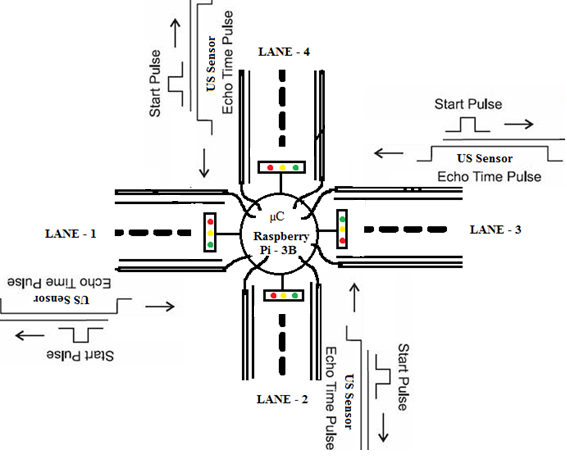
\includegraphics[width=5in]{./images/SystemArchitecture.png}
\caption{Architecture of Smart Traffic Control system using IOT}\label{design}
\end{figure}

\section{System Components}
\subsection{Ultrasonic Sensor}

The above shown HC-SR04 Ultrasonic (US) sensor is a 4-pin module, whose pin names are Vcc, Trigger, Echo and Ground respectively. It is used in many applications where measuring distance or sensing objects are required. The module has two eyes like projects in the front which forms the Ultrasonic transmitter and Receiver. The sensor works with the simple formula,

\begin{tabular}{lcr}
Distance &= Speed × Time & (3.1)\\
\end{tabular}
\begin{figure}[h]\centering
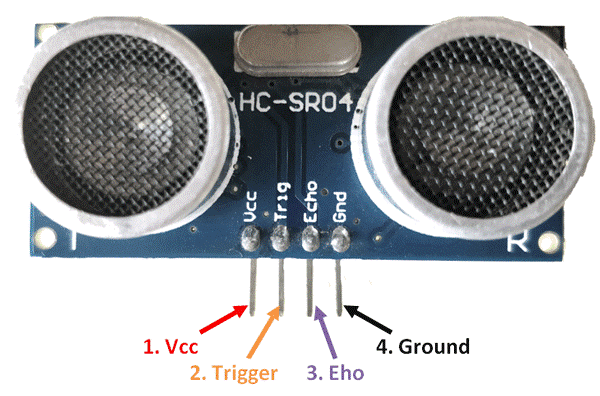
\includegraphics[width=2.5in]{./images/USsensor.png}
\caption{HC-SR04 Ultrasonic Sensor}\label{USsensor}
\end{figure}


The Ultrasonic transmitter transmits an ultrasonic wave, this wave travels in air and when it gets objected by any material it gets reflected back toward the sensor this reflected wave is observed by the Ultrasonic receiver module as shown in the figure \ref{USsensorWorking}

\begin{figure}[h]\centering
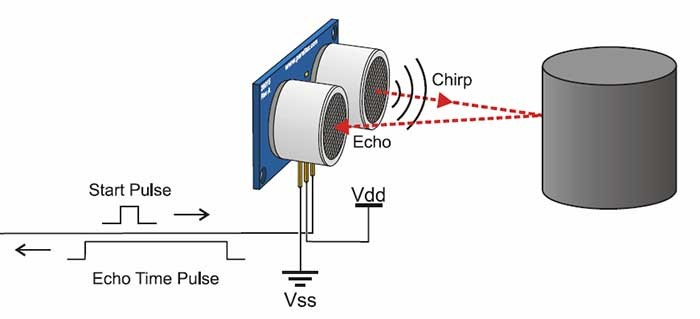
\includegraphics[width=5in]{./images/USsensorWorking.jpg}
\caption{HC-SR04 Ultrasonic Sensor Working}\label{USsensorWorking}
\end{figure}

Now, to calculate the distance using the above formula, we should know the Speed and time. Since the Ultrasonic wave is used, we know the universal speed of US wave at room conditions, which is 330m/s. The circuitry inbuilt on the module will calculate the time taken for the US wave to come back and turns on the echo pin high for that same particular amount of time, this way the time taken is known. Now the distance is calculated using the RPi microcontroller.

\pagebreak

\subsection{Raspberry Pi – 3B}

\begin{figure}[h]\centering
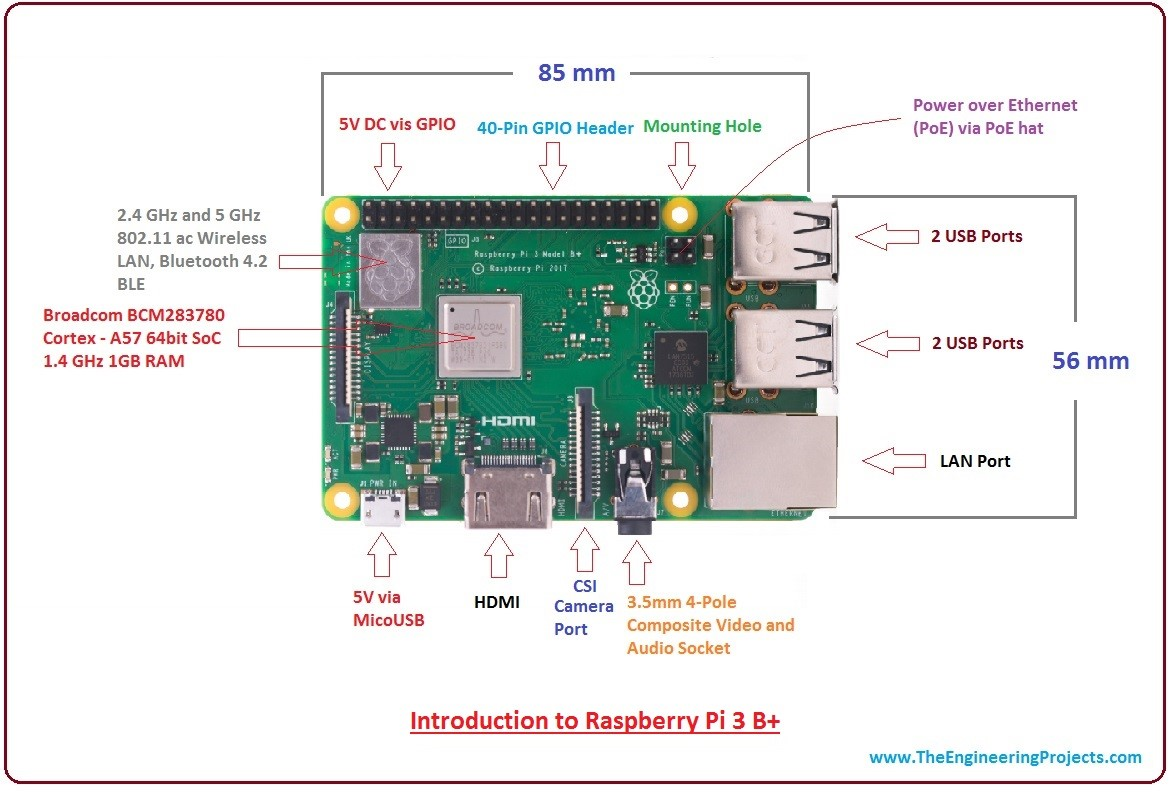
\includegraphics[width=5.5in]{./images/RaspberryPi.jpg}
\caption{Raspberry Pi - 3B}\label{RaspberryPi}
\end{figure}

Raspberry Pi – 3 is a development board in PI series. It can be considered as a single board computer that works on LINUX operating system. The board not only has tons of features it also has terrific processing speed making it suitable for advanced applications, who are interested in LINUX systems and IOT (Internet of Things).

All models feature a Broadcom system on a chip (SoC) with an integrated ARM-compatible central processing unit (CPU) and on-chip graphics processing unit (GPU).

The boards have one to five USB ports. For video output, HDMI and composite video are supported, with a standard 3.5 mm tip-ring-sleeve jack for audio output. Lower-level output is provided by a number of GPIO pins, which support common protocols like I²C. The B-models have an 8P8C Ethernet port and the Pi 3, Pi 4 and Pi Zero W have on-board Wi-Fi 802.11n and Bluetooth.

\pagebreak % adds the Project Design
\chapter{Implementation}
\section{Methodology}

\begin{figure}[h]\centering
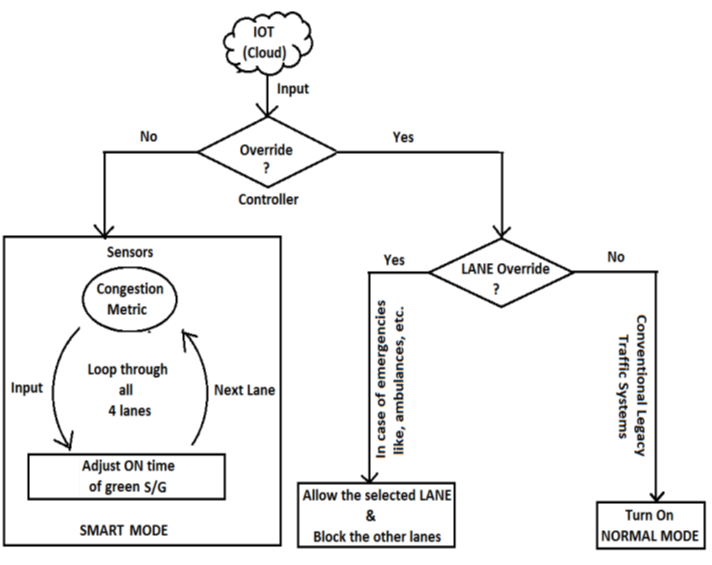
\includegraphics[width=5.5in]{./images/SystemDesign.png}
\caption{Block Diagram of Smart Traffic Control system using IOT}\label{SystemDesign}
\end{figure}
The proposed system mainly operates in two modes,
\begin{itemize}
    \item SMART mode
    \item NORMAL mode
\end{itemize}

\pagebreak

\subsection{SMART MODE}
In SMART mode, the system measures the traffic congestion of a particular lane, by using ultrasonic sensors, in REAL-TIME. The traffic congestion is measured in terms of the distance till which the vehicles are stacked in that lane, which is in direct correlation with the traffic present in that respective lane. The distance is measured using the US sensor with the help of equation 3.1, which can be further simplified down as,

Distance = ((echo pulse period × velocity of sound (330m/s))/2 (4.1)

Here, the distance measured is divided by two since the time for which echo pulse is high is the duration from transmission of ultrasonic signal to it being received back by the sensor after reflecting back from the obstacle. Since, it includes both to and fro motion, the calculated distance is twice that of the distance between sensor and the obstacle. Thus, the measured distance is divided by 2 to get the actual distance.

Once the distance, that gives the measure of congestion of a lane is calculated, the amount of time for which that particular lane vehicles are to be allowed is estimated using an internal algorithm.

\vspace{1cm}

\textbf{Green Time Estimation Algorithm Using Distance}

The basic idea of the algorithm is to estimate time for which the green signal is to be turned on such that, the lane along which there is large congestion/traffic must be allowed for a long time when compared to that of the lane in which the traffic is less. This process ensures that the congestion of the circle is distributed in a balanced manner and equity is given for all lanes.

To accomplish this, a threshold distance and a threshold time is selected (that will be used in case of NORMAL mode), which is the ideal time for which the given lane must be turned on provided, that lane has a traffic corresponding to a distance equal to threshold distance. Based on this setup, now the green time is estimated such that some extra time is added to this threshold value when the actual measured distance is greater than the threshold distance and similarly, some extra time is deducted from the threshold time, when the distance measured is less than the threshold distance.

This extra time that is to be added/subtracted from the threshold value is computed such that it is proportional to the difference in the actual distance and the threshold distance. It is calculated as follows, 

Delta Time = Threshold Time × ((Actual distance – Threshold distance))/(Threshold distance) (4.2)

From the above equation, we see that the value of the (Delta time) > 0, when actual distance measured crosses the threshold and it is < 0, when the actual distance is within the threshold. Now, the final estimated time for which the green time should be turned ON for that particular lane is given by,

Estimated GREEN TIME = Threshold Time + Delta Time (4.3)

From the above equation, we see that, the estimated green time is greater than the threshold value, when the actual distance measured is over-shooting the threshold distance (indicating more traffic density) and is less than the threshold value, when the actual traffic is within the threshold distance. Thus, the estimated green time will be calibrated such that it is proportional to the actual congestion that is being measured in real time and there by operates in an adaptive manner to ensure smooth flow of the traffic.

This process is repeated continuously, in a cyclic manner from LANE-1, LANE-2, LANE-3, LANE-4 and back to LANE-1, using the round-robin method.

\pagebreak

\subsection{NORMAL MODE}

In this mode, the model operates like any other conventional traffic system, where the time for which the green signal is to be turned ON is preset. The system cycles through each lane of the signal with this preset timer value. This value is equal to the threshold time that is used in the SMART mode. The system can be toggled back and forth between these two modes at any time using the toggle switch that is setup with the system. Also, the system can be completely reset, in case of any errors.

\subsection{MANUAL OVERRIDE}

The system can also be controlled using a cloud based android application, that is used to override any particular lane to be turned ON, in case of emergency situations like – ambulances, fire brigades, etc. Once the system enters the override mode, the lane selected will be turned ON and the vehicles in that lane are allowed, until it is turned OFF. Once it is off, the system again comes back into SMART mode and continues to operate in the same way as explained above.

Use of cloud-based application do not need the traffic controller to be present in person at the signal and facilitates control of signals from any place, which proves helpful in life saving situations where the ambulances need to be allowed to pass through without any interruption.

\pagebreak

\section{Working Procedure}

\subsection{Running the Code}

Once the RPi is setup and is in place, we have our development environment setup, which is the IDLE Integrated development environment (IDE) used for programming in python, in which the logic of the system is implemented.

IDLE is the default Python editor that is available on Raspbian. It has a built-in interpreter (REPL), which allows you to run commands one at a time to test code and it only works with Python.

IDLE is the default Python editor that is available on Raspbian. It has a built-in interpreter (REPL), which allows you to run commands one at a time to test code and it only works with Python. It is as shown below,

\begin{figure}[h]\centering
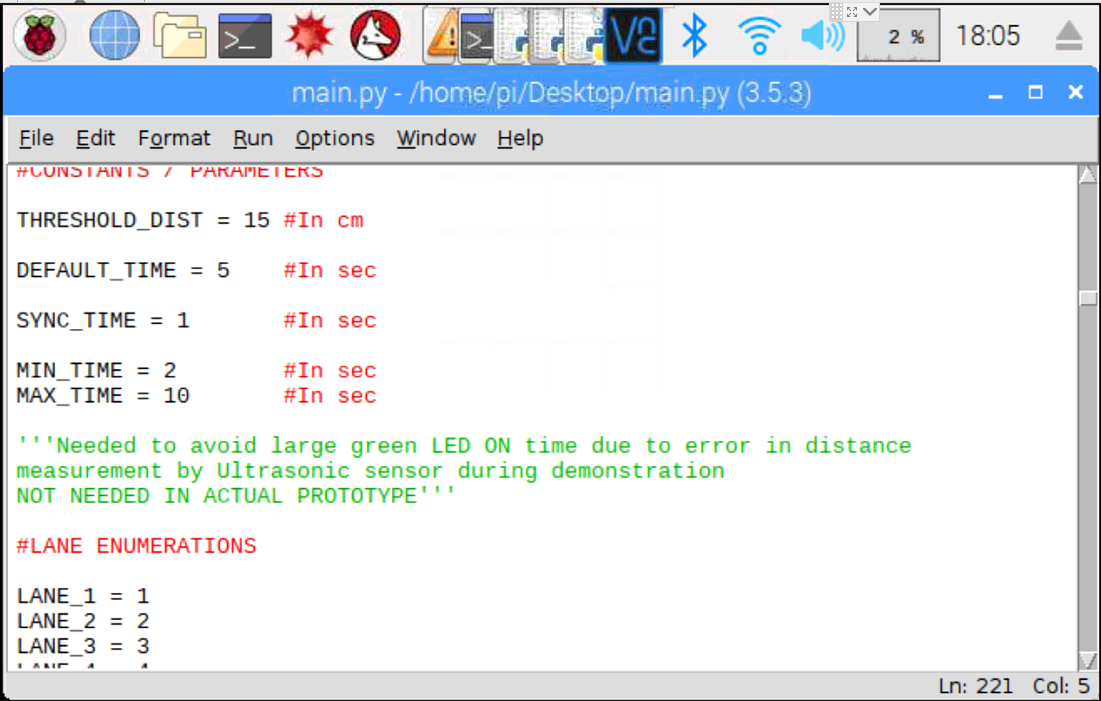
\includegraphics[width=5.5in]{./images/RunningCode.png}
\caption{IDLE IDE for Python}\label{RunningCode}
\end{figure}

Once the peripherals and sensors are connected to the RPI, the code is run with the help of python interpreter, which reads the traffic with the help of US sensor as explained and appropriately calculates the time for which the green signal is to be turned ON using the equations 4.1, 4.2 and 4.3.

\pagebreak

\subsection{Android App Control}

The system also reads the commands from the cloud parallely, to override any particular lane to be turned ON in case of emergencies. An android application is made, which controls the backend cloud data regarding which lane is to be overridden and so. It is powered by Ubidots, which is the most commonly used IOT platform that is used to send or receive data from micro-controllers to server and vice-versa. The android application is also equipped with login-based access to prevent unauthorized usage so as to prevent misuse of the application to control the signals unnecessarily. The lane override interface of the android application that is built is as shown in below figure,

\begin{figure}[h]\centering
        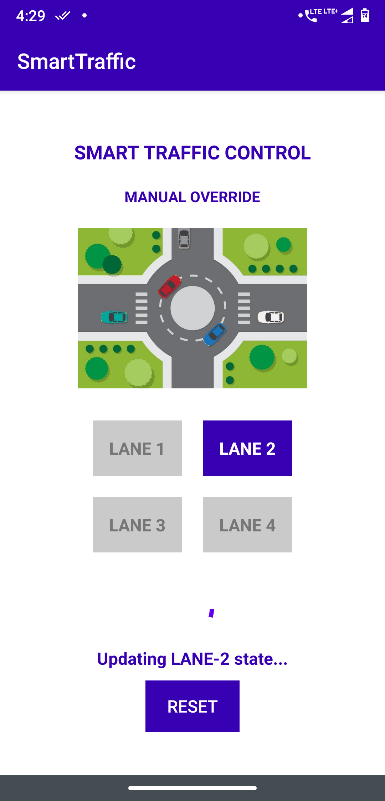
\includegraphics[width=2in]{./images/LaneOverride2.png}
        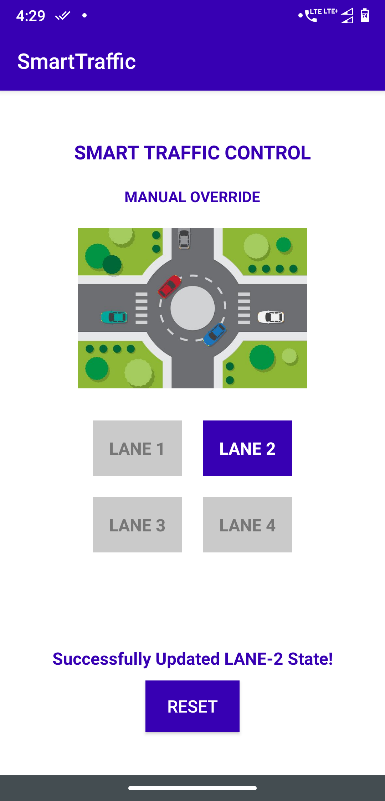
\includegraphics[width=2in]{./images/LaneOverride3.png}
	\caption{SmartTraffic Application - Lane Override}\label{LaneOverrideInterface}
\end{figure}


\pagebreak
 % adds the implementation
\chapter{Result and Output}

\section{Result and Discussion}

The designed system is embedded in the model that emulates a traffic signal and the system is run by dumping the code in the RPi and running the python code. Once the system starts up, it by default enters the SMART mode and the traffic/congestion of each lane is measured and the corresponding time for which the green signal is to be turned ON is estimated depending upon the distance measured and the lane is turned on for the same amount of time. Then, it is switched to the next lane and the same process is repeated once again and then switches to the next lane and so on in a cyclic manner.

Also, the system listens continuously in background, for any update in the cloud for lane overriding which proves useful in case of emergencies. This data is updated and controlled using an android application that controls which lane is to be overridden or whether this feature in itself is to be turned on/off. It is secured using a login-based access, which authenticates only the personnel who has the proper rights to do so. To use this app to control the signal, one has to 1st login to the app by providing proper credentials and then select the lane which is to be turned ON and overridden. This data is stored in the backed powered by Ubidots, which is then sent to the RPi that is controlling the signal, which then takes the corresponding action to override that lane and turns it ON till further notice is received from the cloud (Ubidots) to turn it off, which is again done through the android application.

The system also can be toggled into NORMAL mode and back to SMART mode at any time using the toggle switch by traffic controller at the signal. It also has a reset switch that can be used by the traffic controller to completely reset the system in case of any errors.

\section{Output}

The output of the system running and it being controlled using the android application is documented. The following are the pictures that demonstrate the working of the system and it’s interaction with the cloud and the android application,

\begin{figure}[h]\centering
	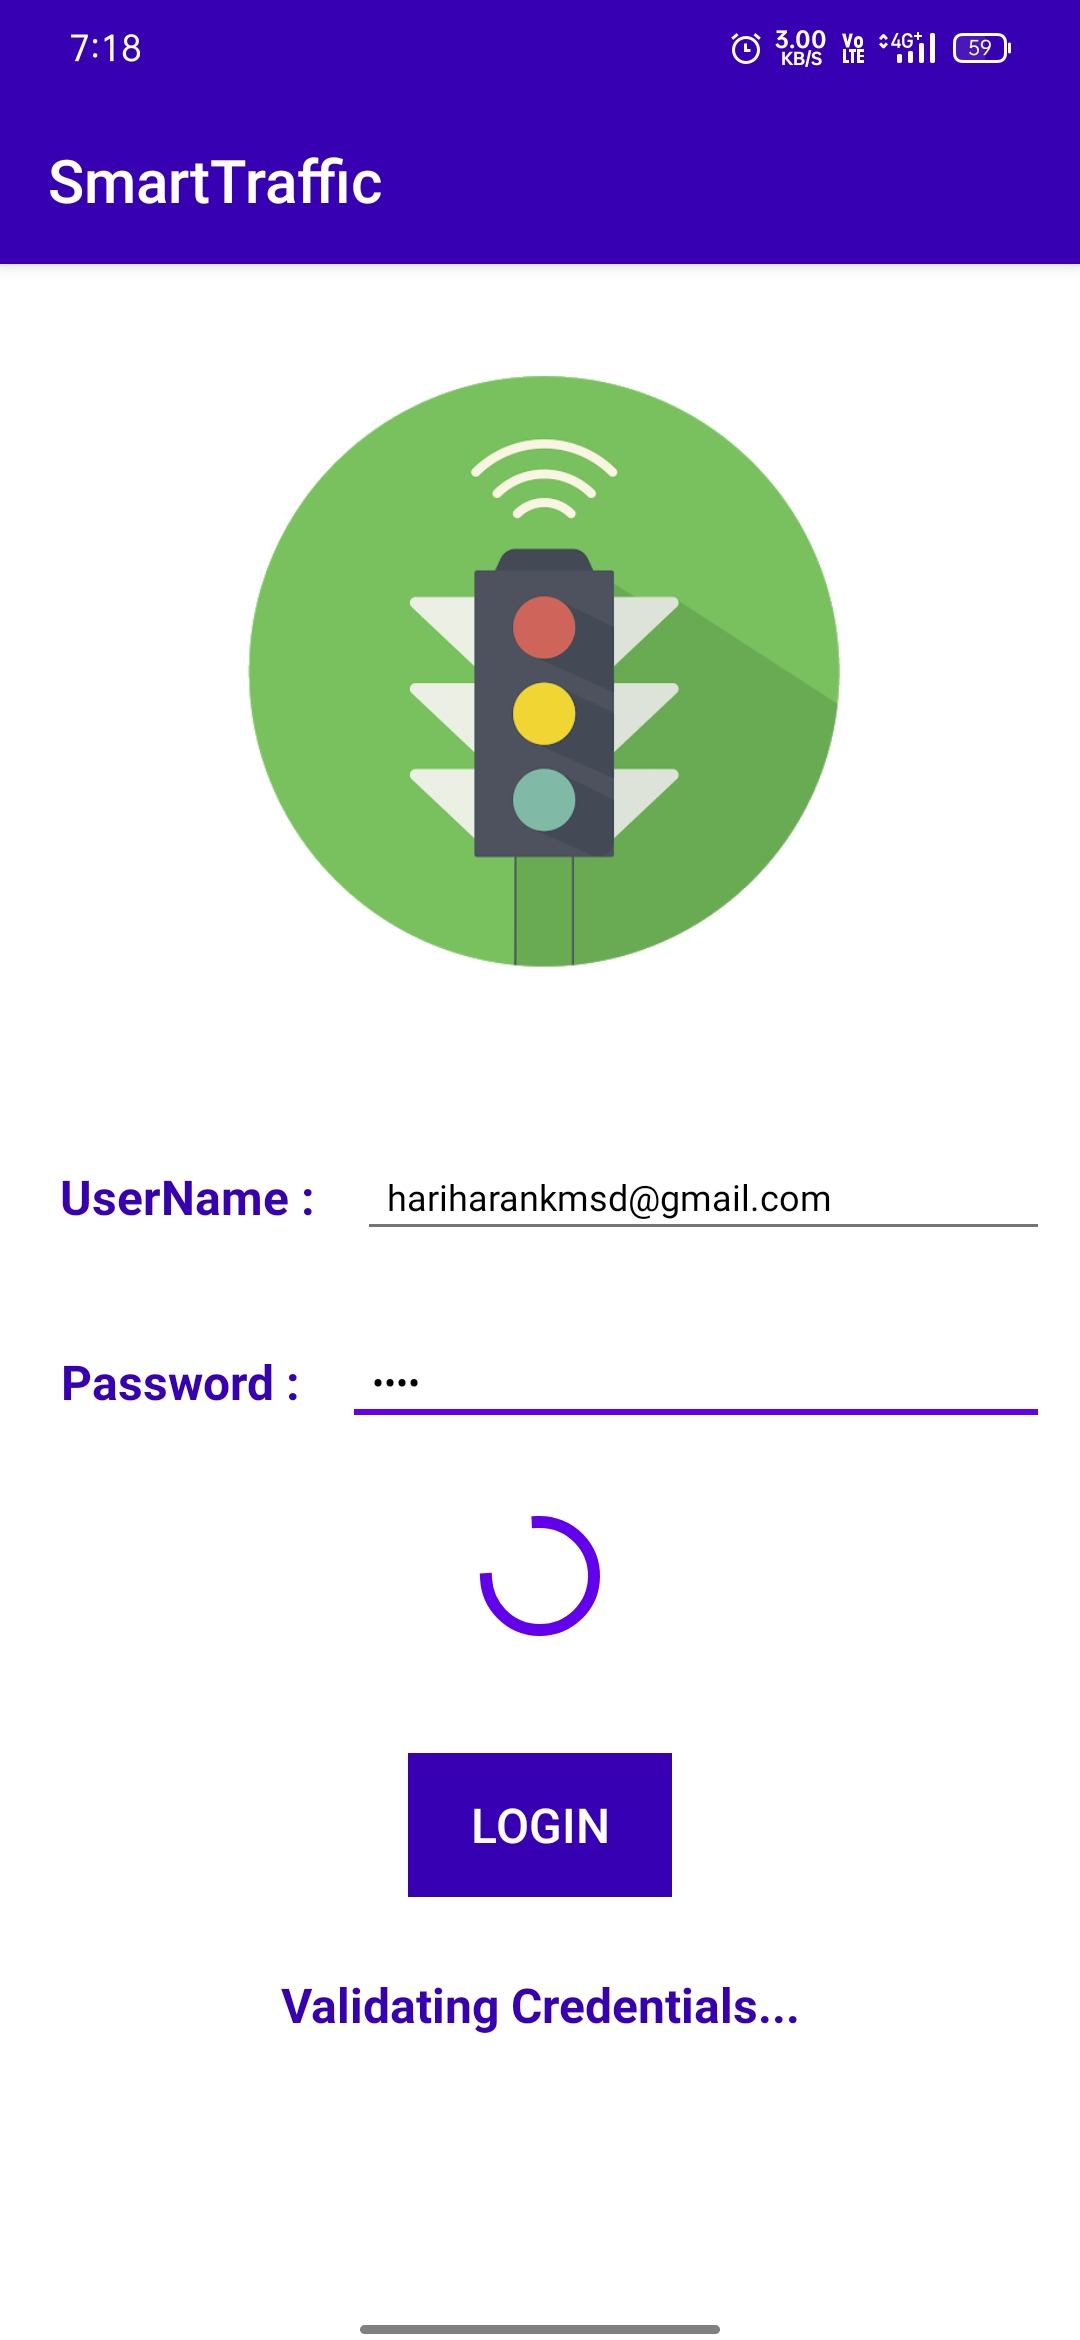
\includegraphics[width=1.75in]{./images/Login1.jpg}
        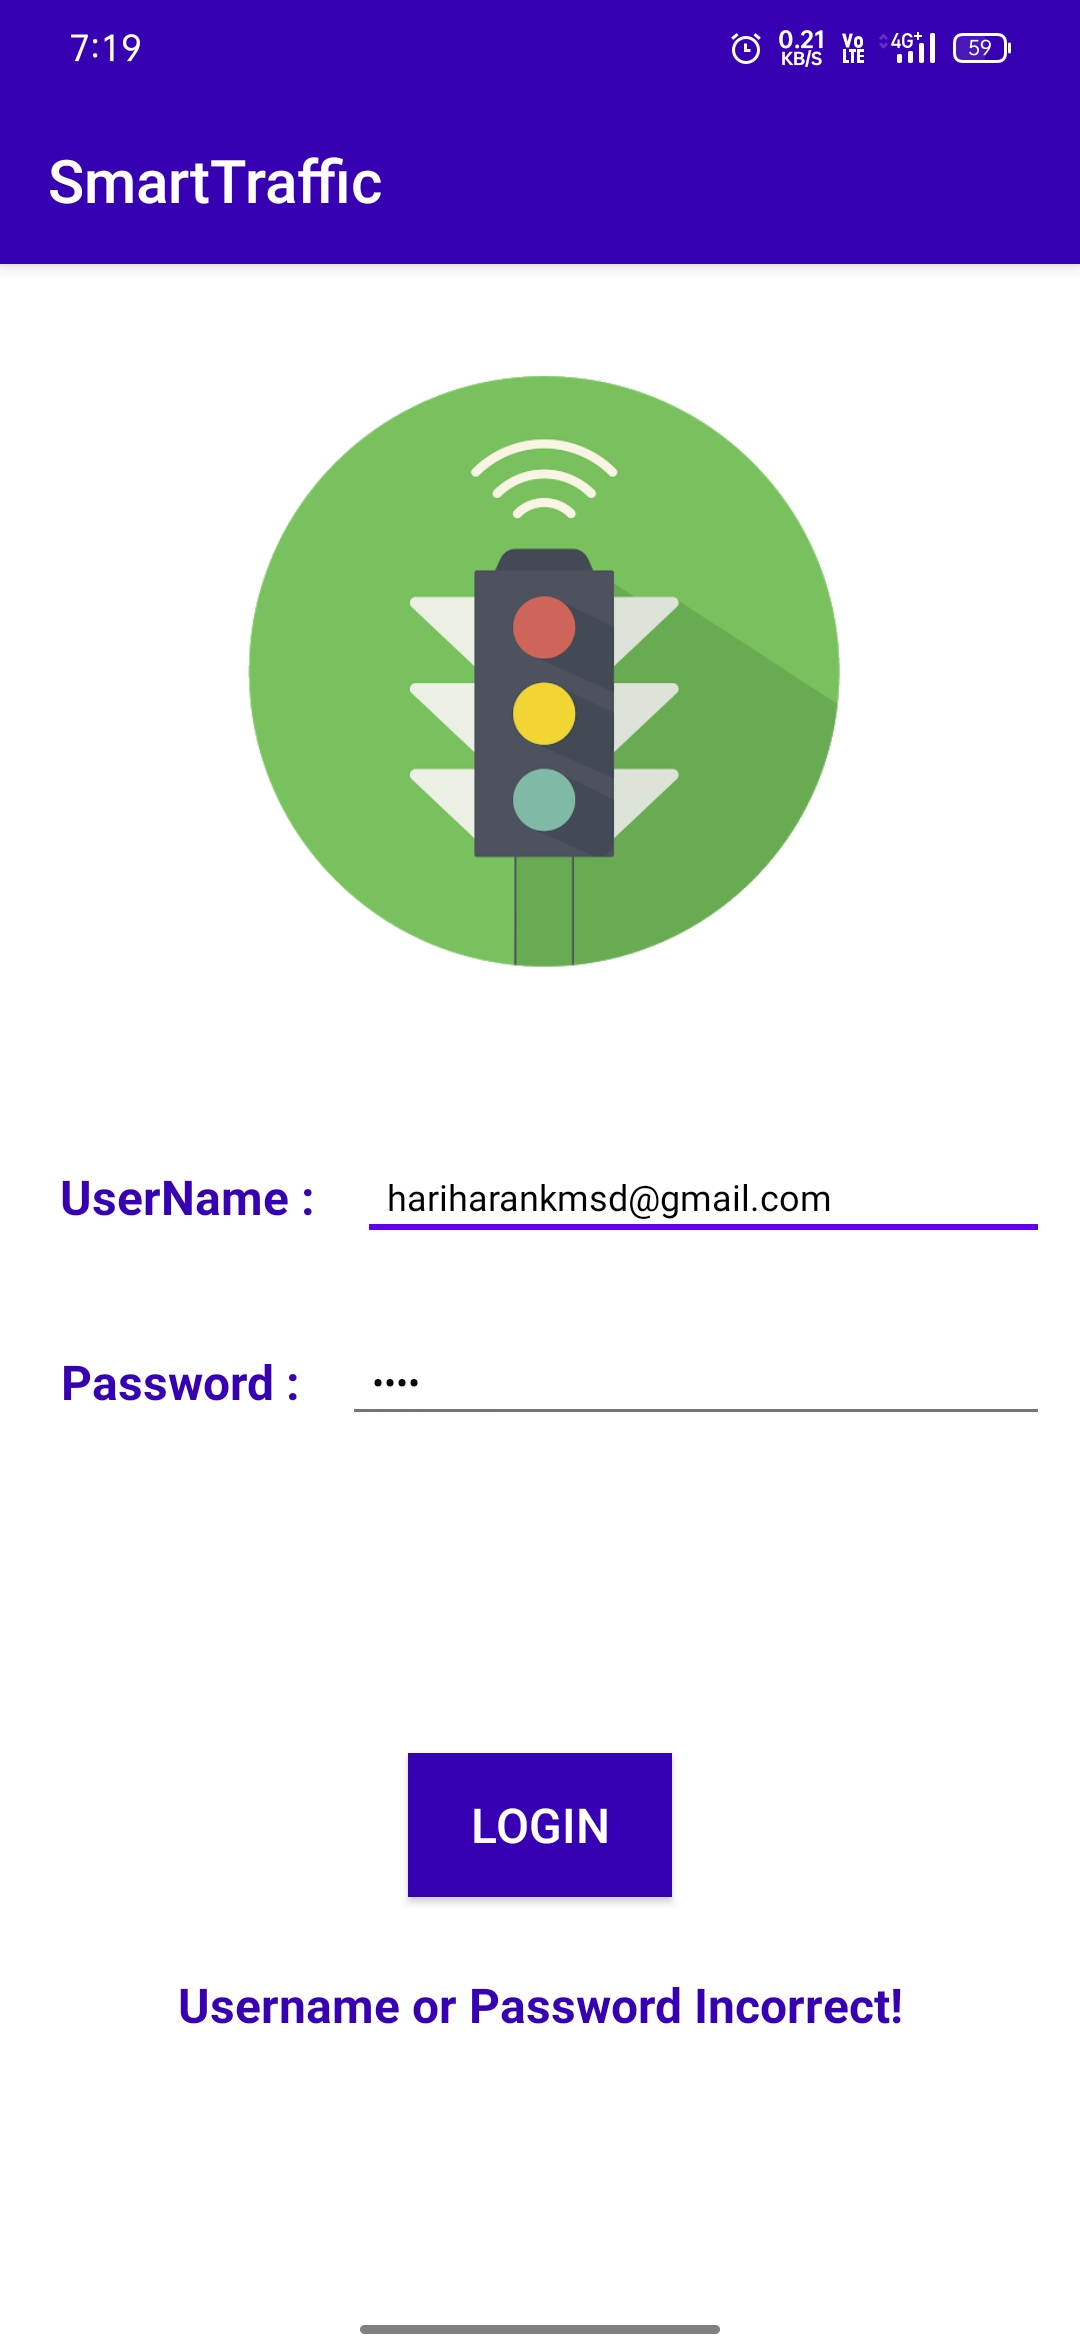
\includegraphics[width=1.75in]{./images/Login2.jpg}
        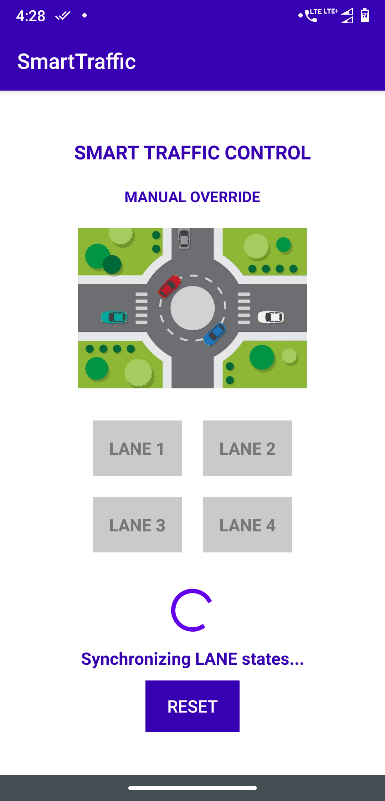
\includegraphics[width=1.75in]{./images/Login3.png}
	\caption{SmartTraffic Application - Login Interface}\label{Login}
\end{figure}

\pagebreak

\begin{figure}[h]\centering
	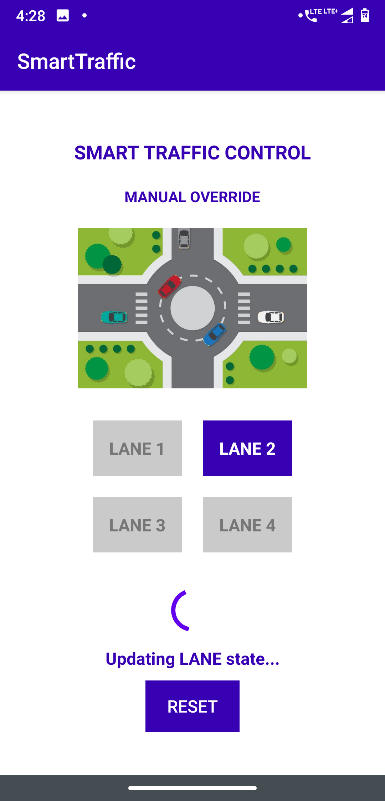
\includegraphics[width=1.75in]{./images/LaneOverride1.png}
        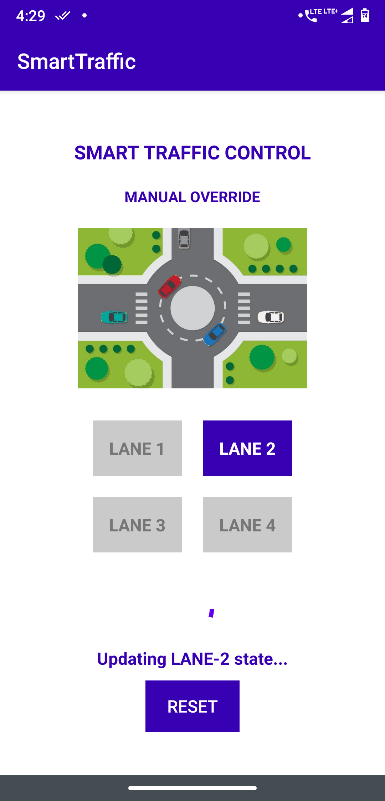
\includegraphics[width=1.75in]{./images/LaneOverride2.png}
        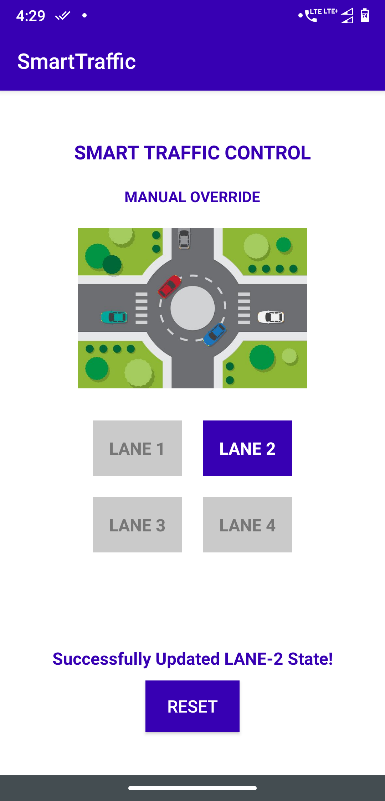
\includegraphics[width=1.75in]{./images/LaneOverride3.png}
	\caption{SmartTraffic Application - Lane Override}\label{LaneOverride}
\end{figure}

From above, we see that the android app covers following functionalities,

\begin{itemize}
    \item Login Authentication and Authorization
    \item Synchronizing the current override states of different lane states
    \item Overriding the lane state of any given lane to ON/OFF
    \item Resetting the Lane Override functionality
\end{itemize}				% adds result page
\chapter{Conclusion and Future Works}

\section{Conclusion}
The aim of the project was to overcome the limitations of the conventional traffic systems where the time for which each lane is allowed to pass through was preset or fixed. The proposed system overcomes this problem by calculating/estimating this time in REAL-TIME depending upon the congestion in that corresponding lane thereby reducing the inflow of the traffic and ensuring proper flow of the vehicles in accordance with the dynamic traffic variations. This Project proves helpful in reducing the time wastage at the traffic signal whenever the traffic is less, since the legacy systems have preset timer values. Along with it, the overriding of the flow of the system by means of the IOT platform through cloud using android based user interface makes it easy for the traffic controller to control the signal from any place without the need for being present in person during emergency situations like – passing of ambulances, fire brigades, etc.

Finally, use of this system proves helpful as it is adaptive and flexible that auto adjusts depending upon the current traffic/congestion, thus overcoming many of the drawbacks of the current conventional traffic systems.

\pagebreak

\section{Future Works}
The proposed model is a 1st step towards making the controlling and handling of the traffic in large cities easier and adaptive. The system paves way for numerous possibilities that can be incorporated upon without changing much of the current prototype. Some of them are listed below,
\begin{itemize}
\item Current system is made to be constrained to a single traffic signal or circle. The system might be modified to handle multiple signals of the city through a single endpoint.
\item The linking of system to multiple signals together under a common control might demand the IOT system to be converted to wireless, since the wired connection and linking up all of them together through wired medium might be tedious.
\item Once the system is converted to support communication through wireless means, we can have a way to send the current traffic trends of all the different signals of a city to a common endpoint in cloud and then this data can be used to visualize the complete overview of the traffic in the city and can take necessary measures based on the inference arrived from the data visualization.
\item Also, with the dynamic estimation of green time, we can go on with other lane switching algorithm other than the current round robin method, if the traffic is very high such as – priority switching in which the system is switched to a lane with high congestion more frequently to allow more vehicles to pass through thereby ensuring smooth flow of congestion in all the lanes.
\end{itemize}

\pagebreak
 % adds conclusion page

\pagebreak
% Appendices.
%  \appendix
% \chapter{PDF generation code snippet}\label{code}
The following is the code snippet used to invoice as pdf using dompdf.

%Use verbatim environment to insert code
\begin{verbatim}
<?php
session_start();
include 'Invoice.php';
$invoice = new Invoice();
$invoice->checkLoggedIn();
if(!empty($_GET['invoice_id']) && $_GET['invoice_id']) {
	echo $_GET['invoice_id'];
	$invoiceValues = $invoice->getInvoice($_GET['invoice_id']);		
	$invoiceItems = $invoice->getInvoiceItems($_GET['invoice_id']);		
}
$invoiceDate=date("d/M/Y,H:i:s",
                    strtotime($invoiceValues['order_date']));
$output = '';
$output='<table width="100%" border="1" cellpadding="5" 
            cellspacing="0">
	<tr>
	<td colspan="2" align="center" style="font-size:18px"><b>Invoice</b>
	 </td>
	</tr>
	<tr>
	<td colspan="2">
	<table width="100%" cellpadding="5">
	<tr>
	<td width="65%">
	To,<br />
	<b>RECEIVER (BILL TO)</b><br />
	Name : '.$invoiceValues['order_receiver_name'].'<br /> 
	Billing Address : '.$invoiceValues['order_receiver_address'].'<br />
	</td>
	<td width="35%">         
	Invoice No. : '.$invoiceValues['order_id'].'<br />
	Invoice Date : '.$invoiceDate.'<br />
	</td>
	</tr>
	</table>
	<br />
	<table width="100%" border="1" cellpadding="5" cellspacing="0">
	<tr>
	<th align="left">Sr No.</th>
	<th align="left">Item Code</th>
	<th align="left">Item Name</th>
	<th align="left">Quantity</th>
	<th align="left">Price</th>
	<th align="left">Actual Amt.</th> 
	</tr>';
\end{verbatim}
 

\pagebreak
\addcontentsline{toc}{chapter}{References}
\begin{singlespace}
  \begin{small}
	\bibliographystyle{unsrt} %unsrt - references appear in the order in which they were cited and are labeled with numbers
	\bibliography{references}
  \end{small}
\end{singlespace}
\end{document}